\nomenclature[]{UE4}{Unreal Engine 4}
\nomenclature[]{RAV}{Robotic Aerial Vehicle}
\note{It might make sense to move some of this to the lit. review}

\subsection{Evaluation Criteria}
In order to design the virtual environment, it was important to first identify the criteria that would determine its usefulness. We began with identifying key phenomena that would need to be present, or integrated in future iterations. This was based on an operational scenario that was outlined in the ROCSAFE project specification\cite{rocsafeNUIG}. Numerous operational scenarios are described that represent distinct classes of CBRNe threat; we picked the one that would be most easily modified for general-purpose use.
\note{Not sure how deeply I can discuss rail environment due to potential dissemination level issues. @Michael will need to approve this. Assuming since most of this work is freely available as an executable, it's ok to describe it here.}
%Would be good to expand this description if possible.
A brief description of the scene is as follows. The scene is set in a rural location, with some forest, a twin track rail line, a small town 10Km away with a small road running near to the rail tracks with access to the rail tracks. The conditions are cool and dry, with a light breeze. A train has been derailed and heavy machinery has been used to damage the tracks. Radioactive material in containers has been exposed. It is intended to use autonomous aerial and ground vehicles to remotely survey and document the scene. They will then be used to localize forensic evidence, subsequently leading to remote evidence collection. The result of modelling this scenario using UE4 is shown in figures x - y.%add figures here.

%Should talk about the rad. environment here but not sure of dissemination status.
The core components that the simulation of this scenario requires were identified: 
\note{This is probably the most important part of this chapter}
\begin{itemize}
    \item The ability to place arbitrary realistic virtual representations of physical objects in the scenario in various configurations
    \item The ability to render high-quality images from the scenario from arbitrary locations at arbitrary resolutions.
    \item There must be sufficient detail in the scene to introduce some noise to image processing problems.
    \item Multiple heterogeneous simulated aerial vehicles, with a high-level API for sensing and navigation for each vehicle. The API should not be platform-specific so that different types of vehicle may be considered.
    \item Simulated sensor readings from the aerial vehicles, including position, velocity, altitude, that depend on the state of the aerial vehicle in the environment. For example, if the aerial vehicle is close to a source of radiation, the simulated sensor reading should be high.
    \item Simulation software should have a permissive licence and should permit publications that include details of the software.
    \item The ability to run the simulations at an increased speed without corrupting the fidelity of the sensor/actuator functionality.
    \item The ability to quickly change the configuration of the simulation.
\end{itemize}
\note{More can be added to this list.}

\subsection{Pre-existing tools and softwares}
In order to provide this functionality, it is clear that using existing tools would be desirable, as writing the boiler plate code necessary to implement such complexity would be extensive. Game engines have been increasingly used for simulations of physical phenomena, with a growing interest in niche areas. Examples include generating high-fidelity training data for computer vision algorithms, \cite{QiuUnrealCV:Engine}, deep learning algorithms \cite{GaidonVirtualAnalysis}, automated crowd size estimation algorithms \cite{Lee2018DigitalCrowds} and target tracking algorithms \cite{Mueller2016ATracking}. An overview of game engines and their use in creating simulation software is outlined in section \ref{GameEngineReview}. The overview describes how most modern simulation softwares that use game engine components are mature in their capabilities to model and render physical scenarios, but not all provide good support for the use of robotic vehicles.
\note{want to get across that basic rendering etc. is offered by many platforms, real issue is to find something to work with that can provide support for Remotely Operated Vehicles / Autonomous vehicles}
This meant that an emphasis was placed on choosing software with some capability to implement high-fidelity simulated aerial vehicles as well as basic physics and graphics rendering.
%Specific functionality can commonly be added to games engines using plugins, which are usually specific to an individual games engine. 
Standalone simulation tools were considered alongside tools built on top of game engines. The simulation softwares whose potential use for designing a custom simulation environment for disaster scene management that were investigated are show in table \ref{table:SimulatorComparison}, with more detailed overviews provided in \cite{Ebeid2018ASimulators}.
\note{Might be better off presenting this as a table.
Format could be Simulator | Licence | Implementation Language | Supported OS | Developer | Additional Notes}
%\begin{itemize}
%Provide a brief description of each.
%    \item Gazebo: A free, open-source standalone simulator written in C++. Development began at the University of Southern California, now maintained by the Open Source Robotics Foundation. \cite{Koenig2005DesignSimulator}
%    \item Airsim: A free, open-source C++ plugin for UE4 developed by Microsoft AI \& Research. MIT Licence. \cite{Shah2017AirSim:Vehicles}
%    \item jMAVSim: A free, open-
%    \item HackFlightSim
%    \item RotorS
%    \item Morse
%    \item New Paparazzi Simulator
%\end{itemize}

\begin{center}
\begin{table}
\footnotesize
\centering
\begin{tabular}{ p{2.1cm} p{2.2cm} p{2.1cm} p{2.1cm} p{2.1cm} p{2.1cm}} 
\hline
Simulator & Implementation Language & Supported OS & Licence & Developer & High-Level Dependencies\\
\hline
Gazebo \cite{Koenig2005DesignSimulator} & C++ & Linux, MacOS & Apache V2.0 & Open Source Robotics Foundation & \\
\\
AirSim \cite{Shah2017AirSim:Vehicles} & C++ & Windows, Linux & MIT & Microsoft & Unreal Engine 4\\ 
\\
jMAVSim \cite{jMAVSim} & Java & Linux, MacOS, Windows & BSD 3 & DroneCode Project & Java3D\\
\\
HackFlightSim (renamed MulticoptorSim) \cite{MulticopterSim} & C++ & Linux, Windows & GPL & SimondLevy & Unreal Engine 4 \\
\\
RotorS & C++ & Ubuntu & ASL 2.0 & ETH Zurich & ROS, Gazebo\\
\\
Morse & Python & Linux & BSD & LAAS-CNRS & Blender Game Engine \\
\\
New Paparazzi Simulator & C & Linux, MacOS & GPL v2 & Ecole Nationale de l’ Aviation Civil & JSBSim\\
\hline
\end{tabular}
\caption{Simulator Comparisons, based on \cite{Ebeid2018ASimulators}}
\label{table:SimulatorComparison}
\end{table}
\end{center}

UE4 with the Airsim plugin was chosen to develop the simulation since the documentation for both suggested that it was most suitable in relation to the design requirements/evaluation criteria outlined above.\par

\subsection{Unreal Engine Design Process}
\note{might need to re-word this. This section should be about the design process that was used once Unreal Engine had be determined the platform of choice to develop with}
The design process of any simulation or game using UE4 should follow certain good practices in order to avoid some common pitfalls that can cause serious delays in development. Once a level has been built using UE4, it can be labor-intensive to radically alter it\cite[p.~454]{Rouse2005GamePractice}. This suggests that care should be taken to ensure to plan the design process so that consistent and efficient results can be achieved.

Unfortunately, most material related to design of simulations and games using UE4 are highly qualitative, addressing questions like "what does the player actually want and how can that be delivered?" rather than describing how the process should proceed. Some good level design practices are noted in \cite{Rouse2005GamePractice}, although many are not applicable to the design of a serious simulation. Notable points include:
\begin{enumerate}
    \item Pencil and paper sketches of the level's general layout can be a very good idea in order to avoid the perils of "designing yourself into a corner". As an example, this could manifest itself as underestimating the proximity between two high-level objects (e.g. a hall and a room) which may lead to a large-scale redesign further down the design process.
    \item During the first pass, do not worry overly about textures and geometry, focus on ensuring that the layout is realistic.
    \item Refine the architecture once a realistic layout has been identified
    \item Add basic gameplay once the physical layout has taken shape. This avoids a tight coupling between the two.
    \item The final step will be to refine gameplay and aesthetics.
\end{enumerate}

Using these concepts as a basis, the design process for the simulation environment proceeded roughly as follows, bearing in mind the evaluation criteria identified at the start of the chapter:
\begin{enumerate}
    \item A sketch of the layout was drawn up based on an operational scenario outlined in the ROCSAFE project proposal \cite{rocsafeNUIG}, which is outlined in section x.
    \item The landscape was sculpted and painted using UE4 in-built landscaping tools.
    \item We identified the assets that would be necessary to develop the environment to our specification. These assets were acquired from websites such as 
\href{http://www.cgtrader.com}{CGTrader}\footnote{\href {http://www.cgtrader.com}{https://www.cgtrader.com}}
and 
\href{https://3dwarehouse.sketchup.com/?hl=en}{Google 3D warehouse}\footnote{\href {https://3dwarehouse.sketchup.com/?hl=en}{https://www.3dwarehouse.sketchup.com}}.
\item The assets were imported into \emph{Autodesk 3DS} in order to ensure that textures were of sufficient quality to facilitate the planned image processing on collected images.
\item They were then imported into UE4 as static meshes and placed into the scene according to the sketch. In order to ensure that this process can scale, we ensured that static meshes could be replaced by simply importing a new mesh which retains the position of the original in the environment. 
\item Rendered images were qualitatively evaluated to determine their suitablility.
\item The environment was archived before integrating "gameplay" and dynamics.
\item The Airsim \cite{Shah2017AirSim:Vehicles} plugin was integrated. This step is non-trivial and details of how this was done is outlined in the next section.
\end{enumerate} 
\note{Would be good to discuss some of the challenges met while developing the simulation and how they were overcome}


\subsection{Design Process Without Dynamic Elements}
This process was carried out iteratively and the results of the developed world excluding the dynamic elements are discussed here. Most changes took place in the UE4 Editor\note{maybe cite}. The chronological development of the virtual world is shown in figure \ref{virutalEnvDevelopment}. The figures on the i$_{th}$ row corresponds to the i$_{th}$ distinct version of the physical layout of the virtual world. The first iteration has many flaws that were improved throughout the development process. The major problems were:
\begin{itemize}
    \item Rendered images were of poor quality due to incorrect UV texture mappings %UV mapping is a technique used to "wrap" a 2D image texture onto a 3D mesh. 
    on objects.
    \item Textures are of poor quality and highly uniform.
    \item The layout of the environment is highly uniform. Note that the rail tracks are perfectly straight.
    \item The scene is minimalist and lacking and convincing detail.
\end{itemize}
Although a human may recognise the scene as a derailed train, it does not capture some key aspects identified in the evaluation criteria. In order to be of real value to the ROCSAFE project for tasks such as localizing an object, it was necessary to address these major problems. Improvements are shown from figures x - y. The techniques used to make these improvements are discussed below.

\note{Might be worth making the margins wider for table of images. Also might be worth recording images again with fixed exposure and orientations for consistency. Come back to this once talked about it with Michael and Frank. Different versions of environment listed at bottom of this file.}

\pagebreak
\note{Will ideally have all of these figures on a single page}
\note{Current format is top view, isometric view, side view. This can be changed but will take quite a lot of effort.}
\note{Might be better to have this landscape instead}
\begin{figure}
\label{fig:virutalEnvDevelopment}
\centering
\begin{tabular}{ccc}
\subfloat[caption]{\includegraphics[width = 4.5cm]{Chapters/SimulationEnv/Figs/VirtualEnvV1/TopView1.png}} &
\subfloat[caption]{\includegraphics[width = 4.5cm]{Chapters/SimulationEnv/Figs/VirtualEnvV1/IsometricView1.png}} &
\subfloat[caption]{\includegraphics[width = 4.5cm]{Chapters/SimulationEnv/Figs/VirtualEnvV1/LowView1.png}}\\
%2nd line of images
\subfloat[caption]{\includegraphics[width = 4.5cm]{Chapters/SimulationEnv/Figs/VirtualEnvV2/TopView.png}} &
\subfloat[caption]{\includegraphics[width = 4.5cm]{Chapters/SimulationEnv/Figs/VirtualEnvV2/IsometricView.png}} &
\subfloat[caption]{\includegraphics[width = 4.5cm]{Chapters/SimulationEnv/Figs/VirtualEnvV2/LowView.png}}\\
%3rd line of images
\subfloat[caption]{\includegraphics[width = 4.5cm]{Chapters/SimulationEnv/Figs/VirtualEnvV3/TopView1.png}} &
\subfloat[caption]{\includegraphics[width = 4.5cm]{Chapters/SimulationEnv/Figs/VirtualEnvV3/IsometricView1.png}} &
\subfloat[caption]{\includegraphics[width = 4.5cm]{Chapters/SimulationEnv/Figs/VirtualEnvV3/LowView1.png}}\\
%4thline of images
\subfloat[caption]{\includegraphics[width = 4.5cm]{Chapters/SimulationEnv/Figs/VirtualEnvV4/TopView2.png}} &
\subfloat[caption]{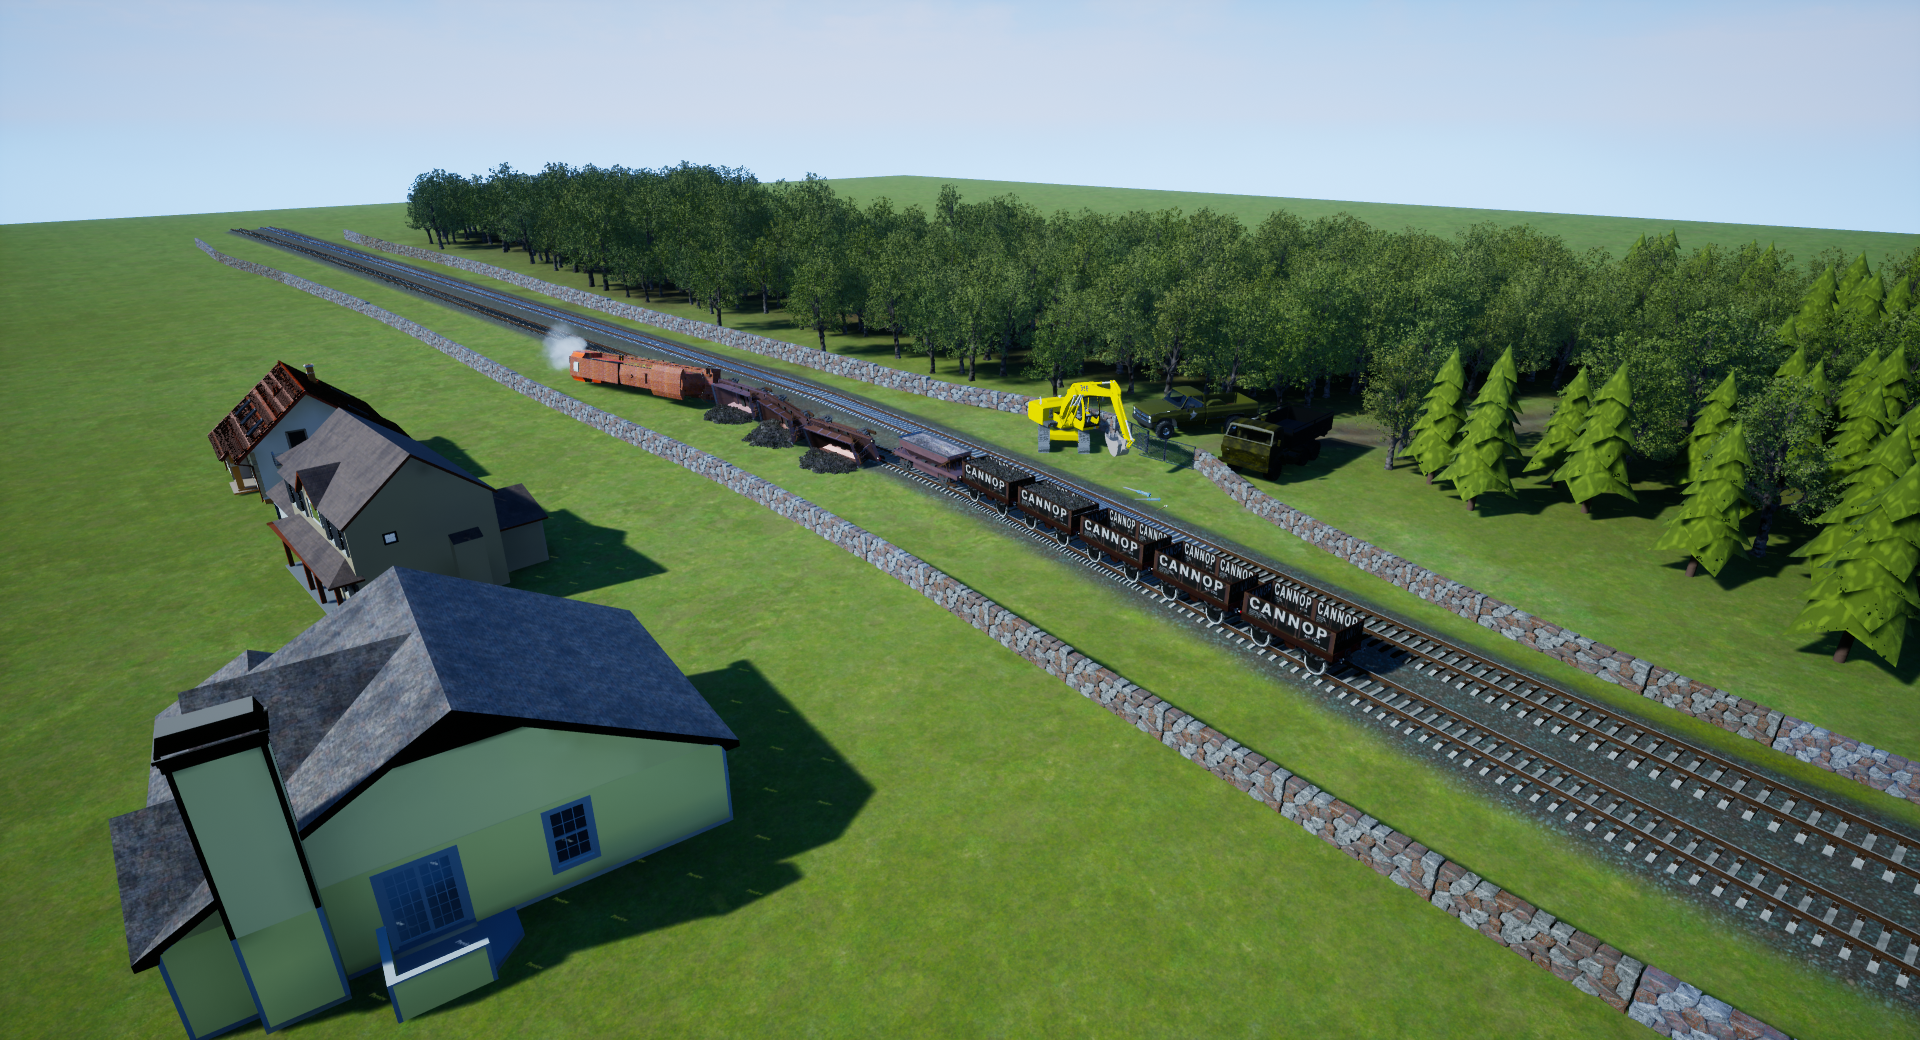
\includegraphics[width = 4.5cm]{Chapters/SimulationEnv/Figs/VirtualEnvV4/IsometricView2.png}} &
\subfloat[caption]{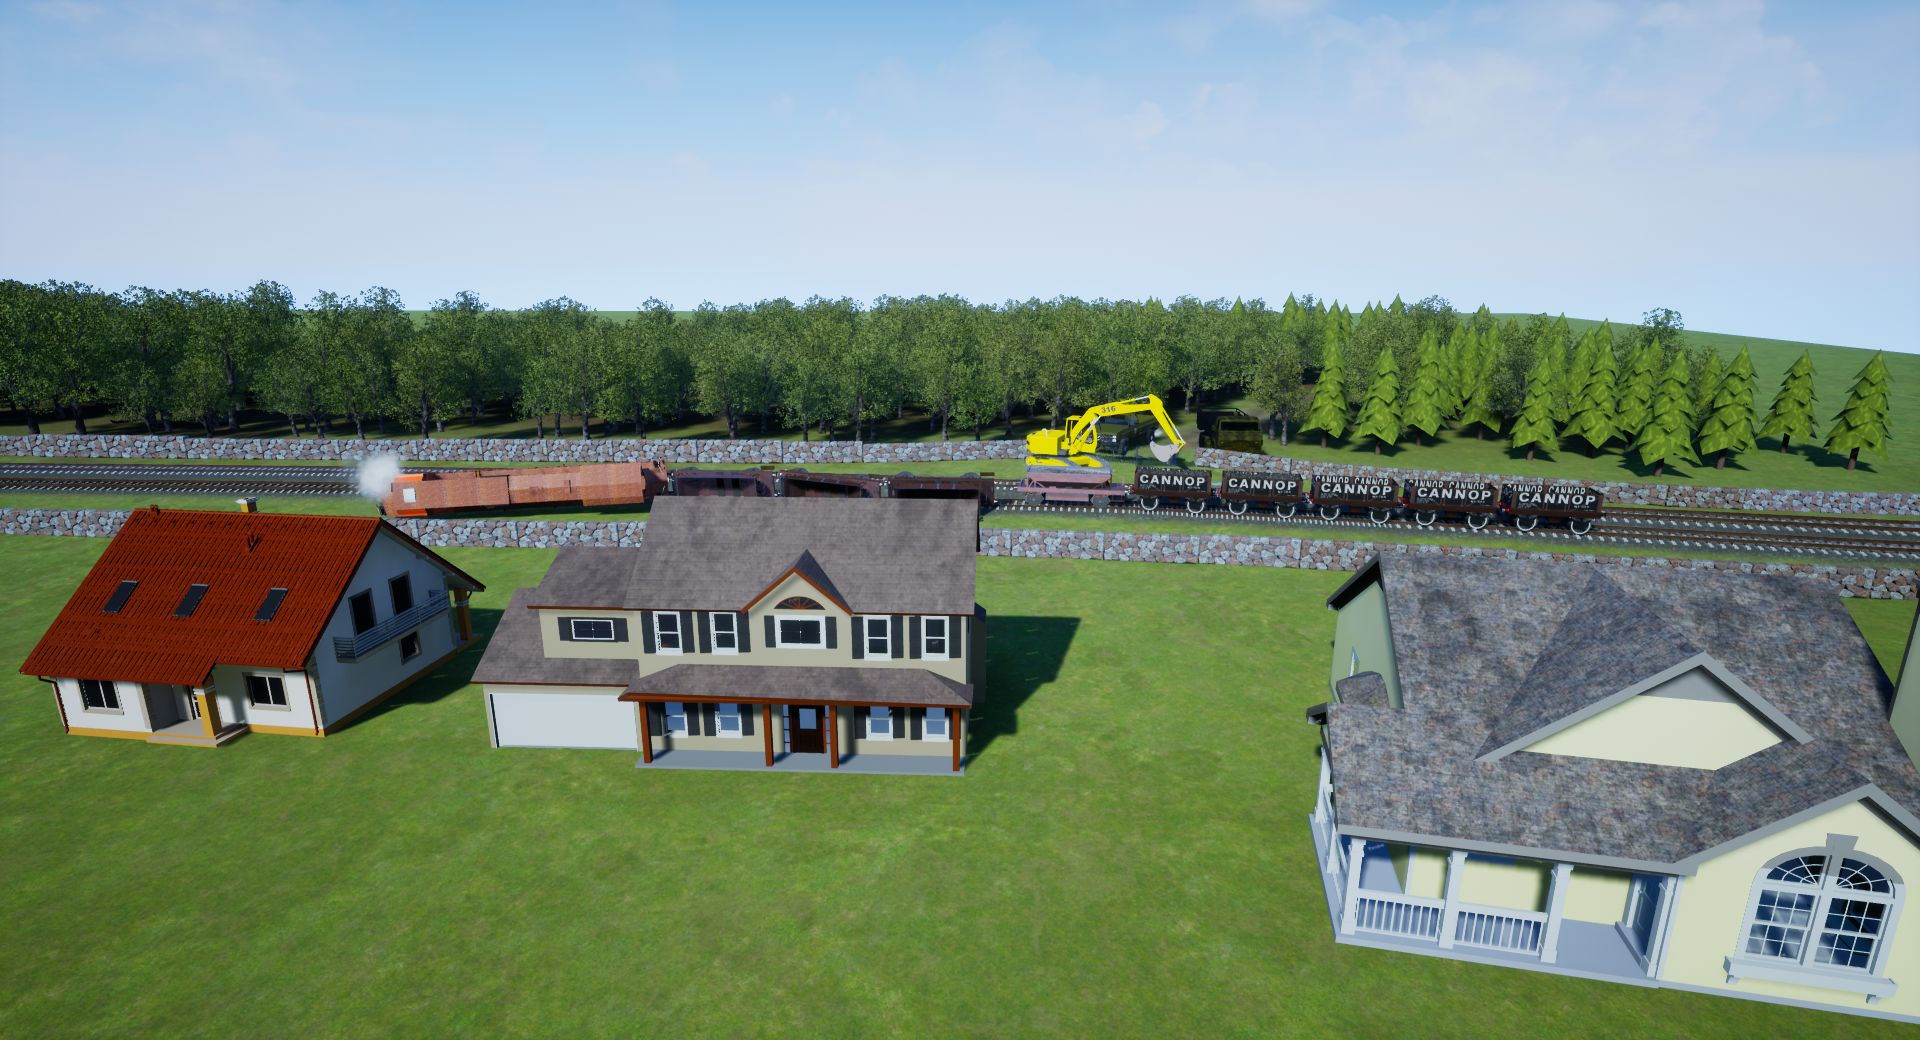
\includegraphics[width = 4.5cm]{Chapters/SimulationEnv/Figs/VirtualEnvV4/LowView2.png}}\\
%5thline of images
\subfloat[caption]{\includegraphics[width = 4.5cm]{Chapters/SimulationEnv/Figs/VirtualEnvV5/TopView.png}} &
\subfloat[caption]{\includegraphics[width = 4.5cm]{Chapters/SimulationEnv/Figs/VirtualEnvV5/IsometricView.png}} &
\subfloat[caption]{\includegraphics[width = 4.5cm]{Chapters/SimulationEnv/Figs/VirtualEnvV5/LowView.png}}
\end{tabular}
\caption{Evolution of Simulation Environment. Each row depicts images from a subsequent iteration.}
\end{figure}
\pagebreak



\note{Might not be necessary to talk about all of these things}

\begin{figure}
\label{fig:virutalEnvDevelopment}
\centering
\begin{tabular}{cc}
\subfloat[caption]{\includegraphics[width = 7cm]{Chapters/SimulationEnv/Figs/VirtualEnvFinal/IsometricView1.png}} &
\subfloat[caption]{\includegraphics[width = 7cm]{Chapters/SimulationEnv/Figs/VirtualEnvFinal/LowView.png}} \\

\subfloat[caption]{\includegraphics[width = 7cm]{Chapters/SimulationEnv/Figs/VirtualEnvFinal/TopView2.png}}&
\subfloat[caption]{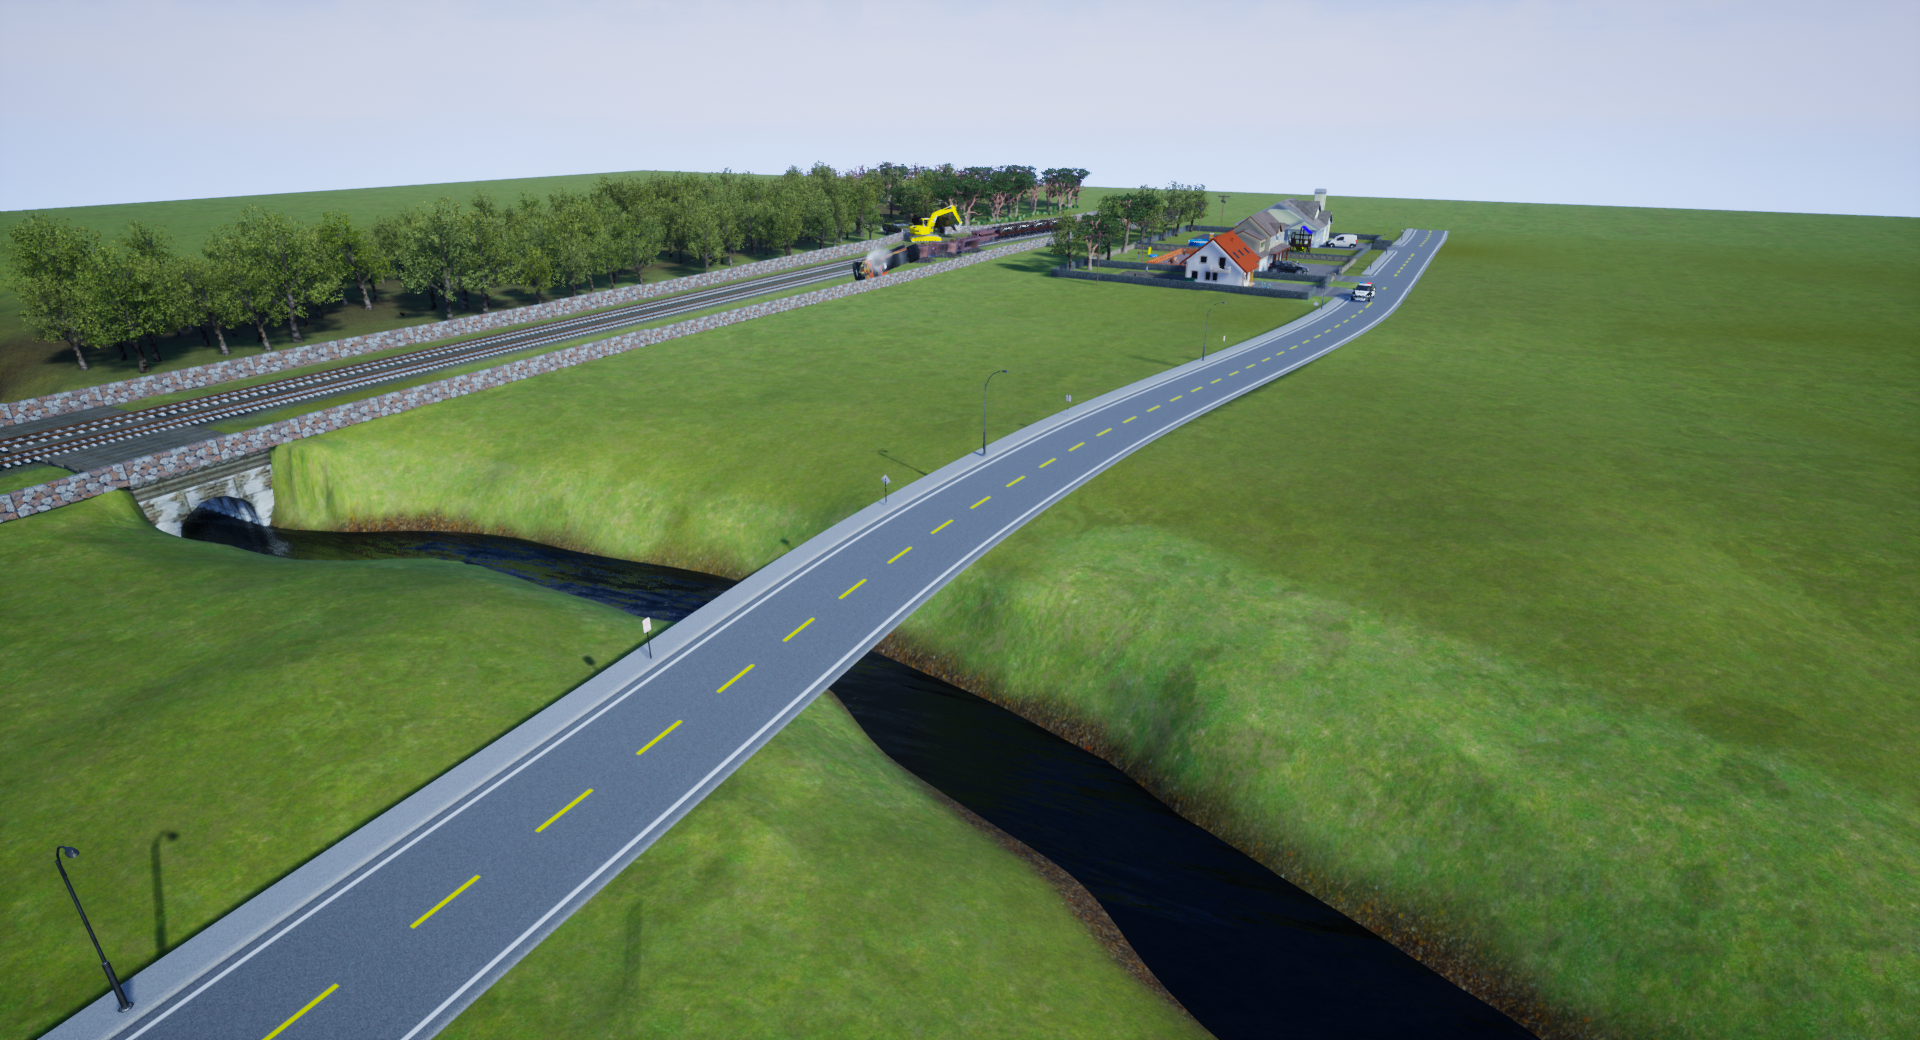
\includegraphics[width = 7cm]{Chapters/SimulationEnv/Figs/VirtualEnvFinal/BridgeView1.png}} \\

\subfloat[caption]{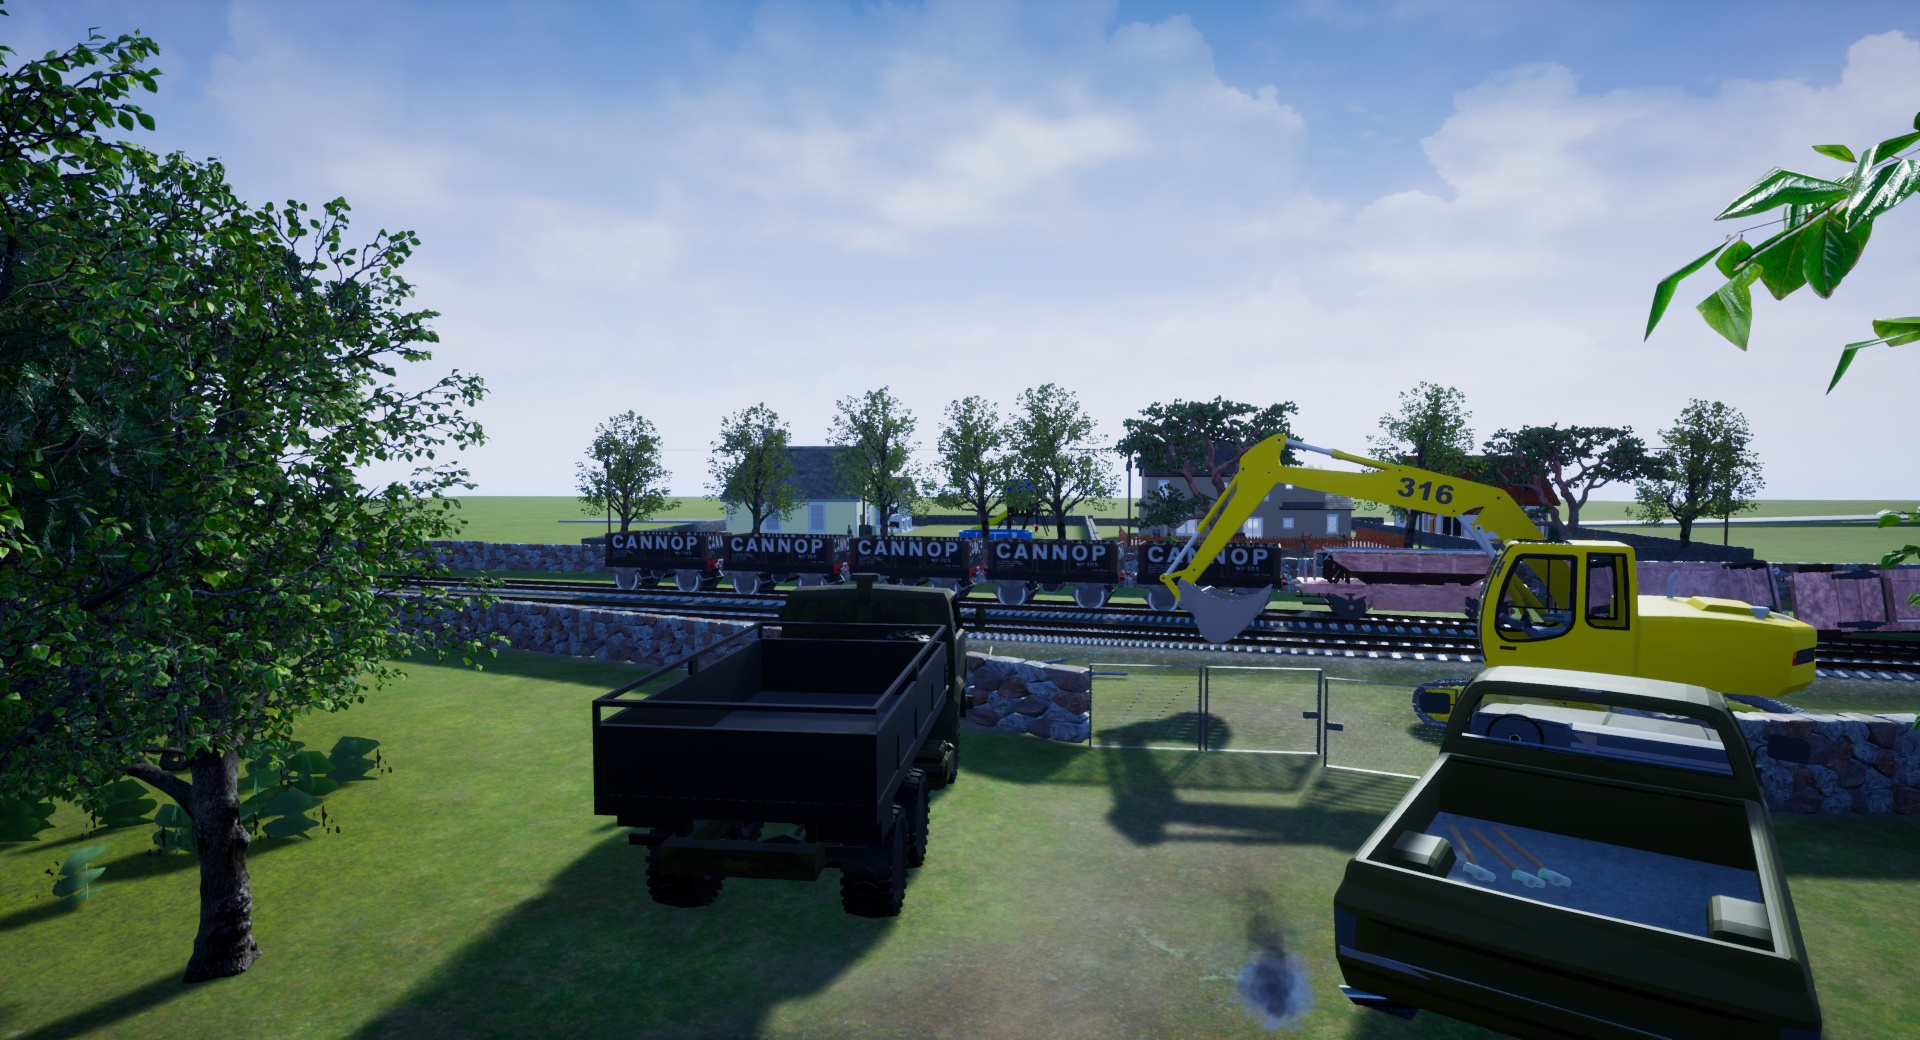
\includegraphics[width = 7cm]{Chapters/SimulationEnv/Figs/VirtualEnvFinal/CloseUp1.png}}&
\subfloat[caption]{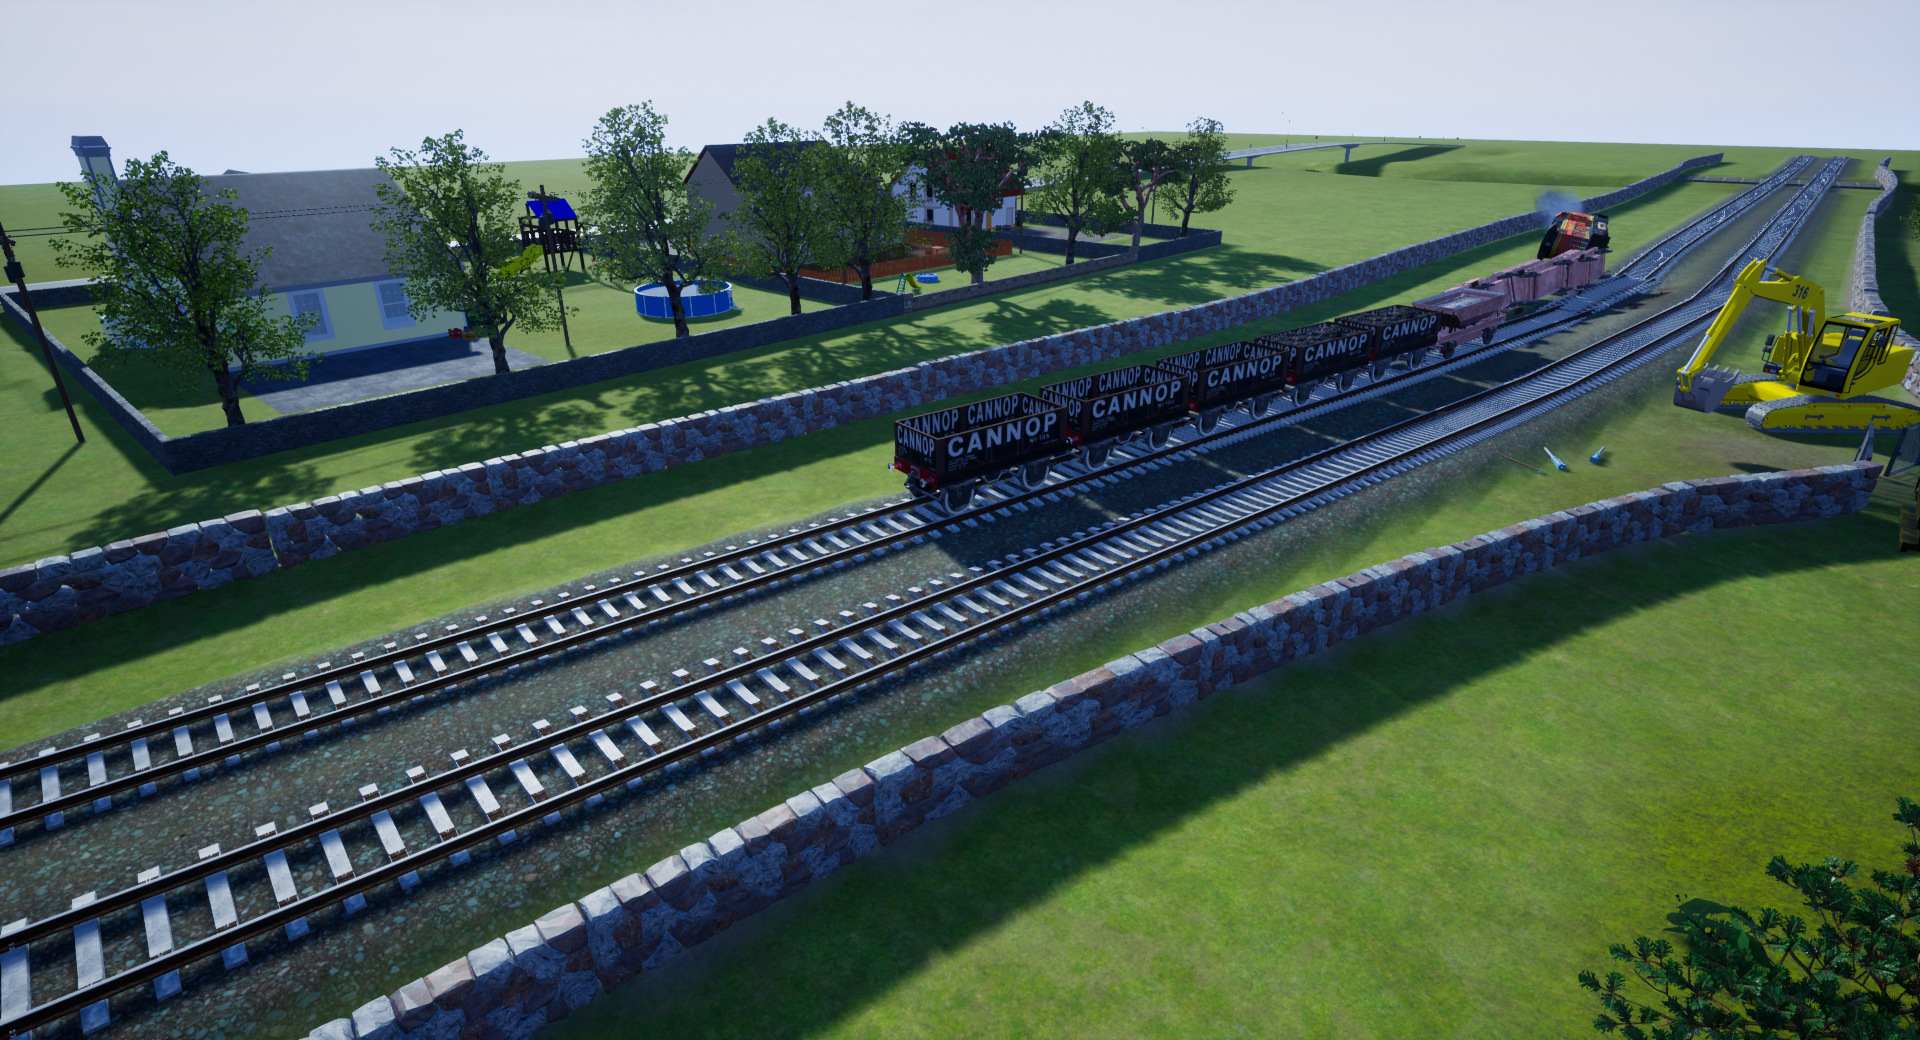
\includegraphics[width = 7cm]{Chapters/SimulationEnv/Figs/VirtualEnvFinal/CloseUp2.png}} \\
\end{tabular}
\caption{Final Version of Simulation Environment}
\end{figure}
\pagebreak

\subsubsection{Blueprint Visual Scripting System}
UE4 uses a visual scripting system to provide a lot of functionality, known as Blueprints. Blueprints provide a node-based interface to create gameplay elements. In order to develop different aspects of a game, the system provides a visual approach to scripting, and many of the tools available in standard written scripting languages are available, such as typed variables, arrays, structs, loops, etc. Blueprints were used extensively in the subsequent sections, as well as C++ code, in order to develop the simulation.


\subsubsection{Materials}
\note{grass, rail tracks}

%\subfloat[caption]{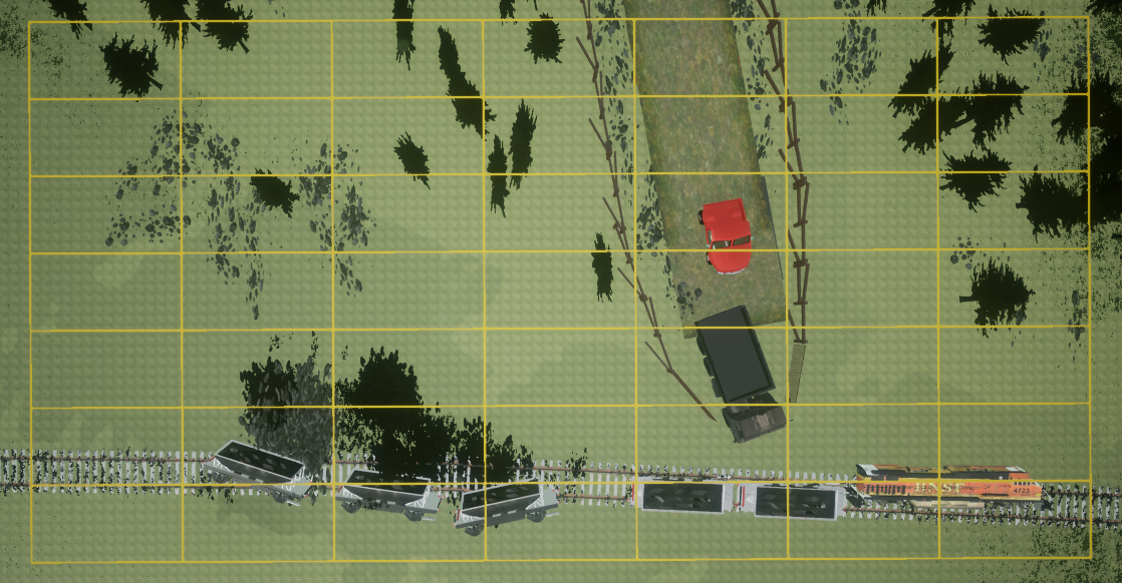
\includegraphics[width = 4.5cm]{Chapters/SimulationEnv/Figs/RailScenarioFirstIteration.png}} &
%\subfloat[caption]{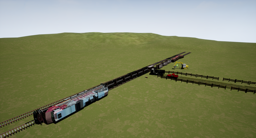
\includegraphics[width = 4.5cm]{Chapters/SimulationEnv/Figs/VirtualEnvV1/resized_HighresScreenshot00001.png}} \\

\begin{wrapfigure}{r}{0.4\textwidth}
    \centering
    \includegraphics[width=0.4\textwidth]{Chapters/SimulationEnv/Figs/BlendedMaterialsVSNotBlendedMaterials/PoorTextures.png}
    \label{fig:PoorTextures}
    \includegraphics[width=0.4\textwidth]{Chapters/SimulationEnv/Figs/BlendedMaterialsVSNotBlendedMaterials/HighQualityMaterial.png}
    \label{fig:GoodTextures}
    \caption{Contrast between initial and final materials used in simulation environment.}
\end{wrapfigure}

%https://docs.unrealengine.com/en-US/Engine/Rendering/Materials/IntroductionToMaterials/index.html
Materials are made up of a number of components in UE4, which specify aspects such as colour, opacity, roughness, specularity and emissive colours. In order to produce realistic materials, it is necessary to blend and layer different textures as well as identifying the correct parameters for surface normals and specularity, among the other features. UE4 has highly sophisticated tools for modifying materials to achieve a high-fidelity output. Details of creating materials can be found in the 
\href{https://docs.unrealengine.com/en-US/Engine/Rendering/Materials/IntroductionToMaterials/index.html}{UE4 Documentation}\footnote{\href {https://docs.unrealengine.com/en-US/Engine/Rendering/Materials/IntroductionToMaterials/index.html}{https://docs.unrealengine.com/en-US/Engine/Rendering/Materials/IntroductionToMaterials/index.html}}. The landscape in the first iteration of the virtual environment consisted of a single uniform texture, with none of the parameters mentioned above properly specified. The result of this is shown in figure \ref{fig:PoorTextures}. Subsequent versions used multiple layers and blending in order to create a higher-fidelity material, with relevant parameters tuned. This is shown in figures \ref{fig:LayerBlendNode} and \ref{fig:LandscapeMaterialBlueprint}, where a Landscape Layer Blend node is used to combine individual textures to create the landscape material.

\begin{figure}
\centering
\begin{tabular}{cc}
\subfloat[Layers blended into Landscape Layer Blend Node]{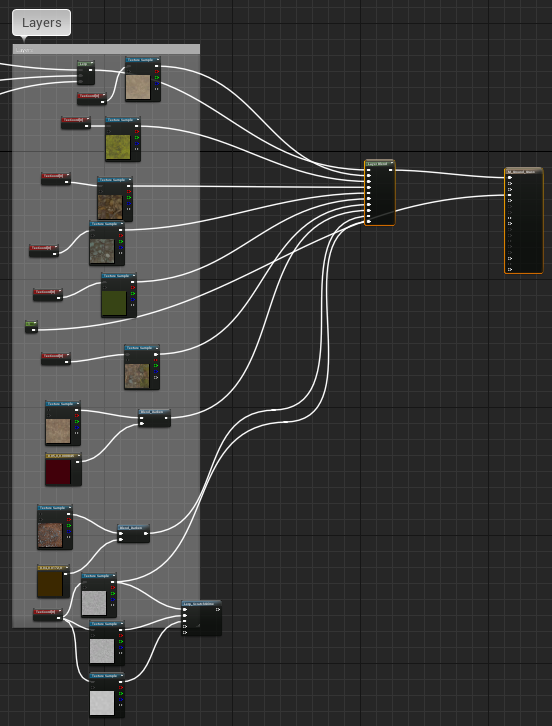
\includegraphics[width=4cm]{Chapters/SimulationEnv/Figs/BlendedMaterialsVSNotBlendedMaterials/LayerBlend.PNG}}\label{fig:LayerBlendNode} &


\subfloat[Blueprint used to create landscape material]{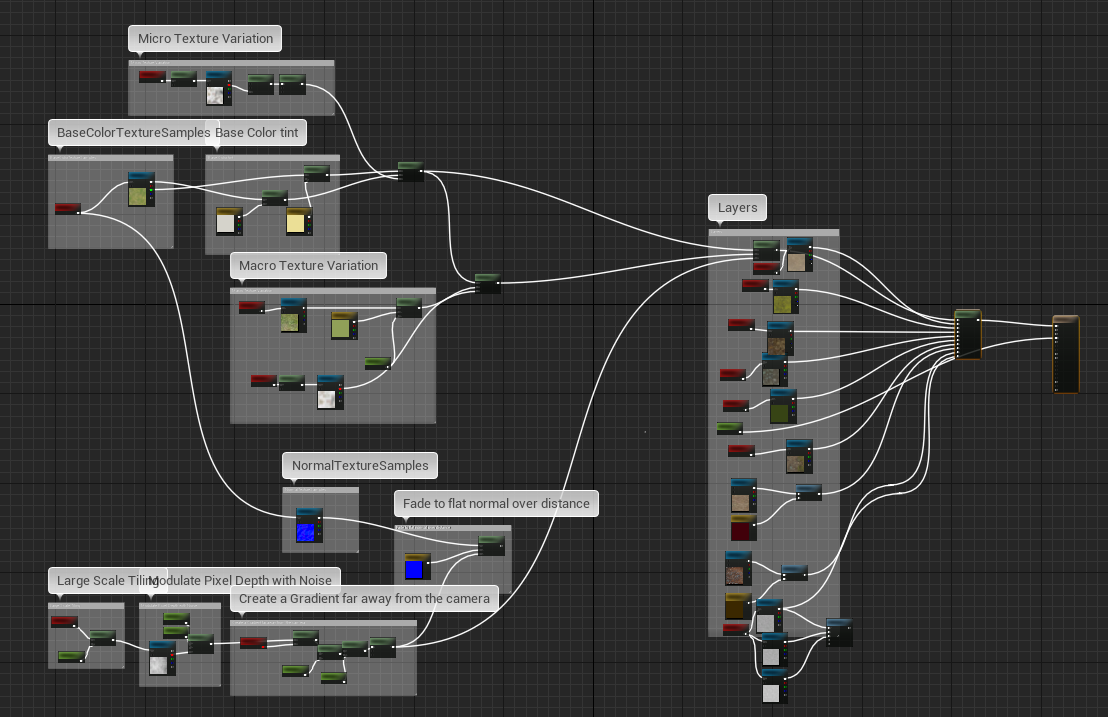
\includegraphics[width=4cm]{Chapters/SimulationEnv/Figs/BlendedMaterialsVSNotBlendedMaterials/LandscapeMaterial.PNG}}\label{fig:LandscapeMaterialBlueprint}
\end{tabular}
\caption{test}
\end{figure}


\subsubsection{Splines}

\begin{wrapfigure}{r}{0.4\textwidth}
    \centering
    \includegraphics[width=0.4\textwidth]{Chapters/SimulationEnv/Figs/SplineVSNoSplineExamples/PerfectlyStraightRail.png}
    \label{fig:StraightRail}
    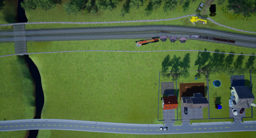
\includegraphics[width=0.4\textwidth]{Chapters/SimulationEnv/Figs/SplineVSNoSplineExamples/resized_SplineExample1.png}
    \label{fig:SplinedRail}
    \caption{Contrast between initial and final materials used in simulation environment.}
    
\end{wrapfigure}

Uniformity tends to be rare in the real world; perfectly straight lines don't often occur naturally. For this reason UE4 offers tools to create splines, along which the terrain can be deformed. Splines are typically used to model roads and paths, but the Landscape Spline system is very flexible and can be used to model many different phenomena. In the initial stages of the simulation environment, only a perfectly straight section of rail could sourced for use in the environment, as shown in figure \ref{fig:StraightRail}. The spline tool allowed for much more realistic construction of the section of rail and accompanying wall, as shown in figure \ref{fig:SplinedRail}. It was also used to create the road and the bridge section. \note{maybe provide link to docs}


\subsubsection{Foliage}
Similar to the argument made in relation to splines, it is rare to have uniformly configured foliage in the real world. In order to address this, there exist foliage generation and editing tools in UE4 editor. Version 4.18 of the editor onwards contains the Procedural Foliage Tool \note{maybe add a link}, which is the most convenient way to add swathes of foliage to a scene. Since we were using other content dependent on UE 4.16, we opted to use the foliage painter tool, which allows the user to effectively paint foliage directly onto a landscape. It allows the user to specify a number of parameters to achieve the required density, scaling and other relevant features. The results of applying foliage to the scene are visible in figures \ref{}, \ref{} and \ref{} respectively.
\note{Non-uniform trees, grass, etc.}

\begin{figure}
\centering
\begin{tabular}{ccc} 
\subfloat[Layers blended into Landscape Layer Blend Node]{\includegraphics[width=4cm]{Chapters/SimulationEnv/Figs/Foliage/Foliage2.png}}\label{fig:LayerBlendNode} &

\subfloat[Blueprint used to create landscape material]{\includegraphics[width=4cm]{Chapters/SimulationEnv/Figs/Foliage/Foliage5.png}}\label{fig:LandscapeMaterialBlueprint} &
\subfloat[Blueprint used to create landscape material]{\includegraphics[width=4cm]{Chapters/SimulationEnv/Figs/Foliage/Foliage6.png}}\label{fig:LandscapeMaterialBlueprint}
\end{tabular}
\caption{test}
\end{figure}

\subsubsection{Landscape Editing}
\note{Discuss here how dirt track was created using}
Creating a realistic landscape in UE4 serves a number of purposes. In order to allow the potential simulation of the operation of ground vehicles, it is necessary to model the terrain realistically so that difficulties that may be experienced in the real world, such as steep climbs or highly uneven surfaces, may be taken into account. UE4 provides a suite of landscaping tools that allows the user to create a highly variable landscape. The tools facilitate raising and flattening, smoothing, random noise and simulated erosion, as well as allowing for other more detailed modifications. These were used to create the railway embankment, the rutted path leading onto the rail tracks and the riverbank and riverbed, shown in figures \ref{}, \ref{} and \ref{} respectively.

\begin{figure}
\centering
\begin{tabular}{ccc}
\subfloat[Rutted Track]{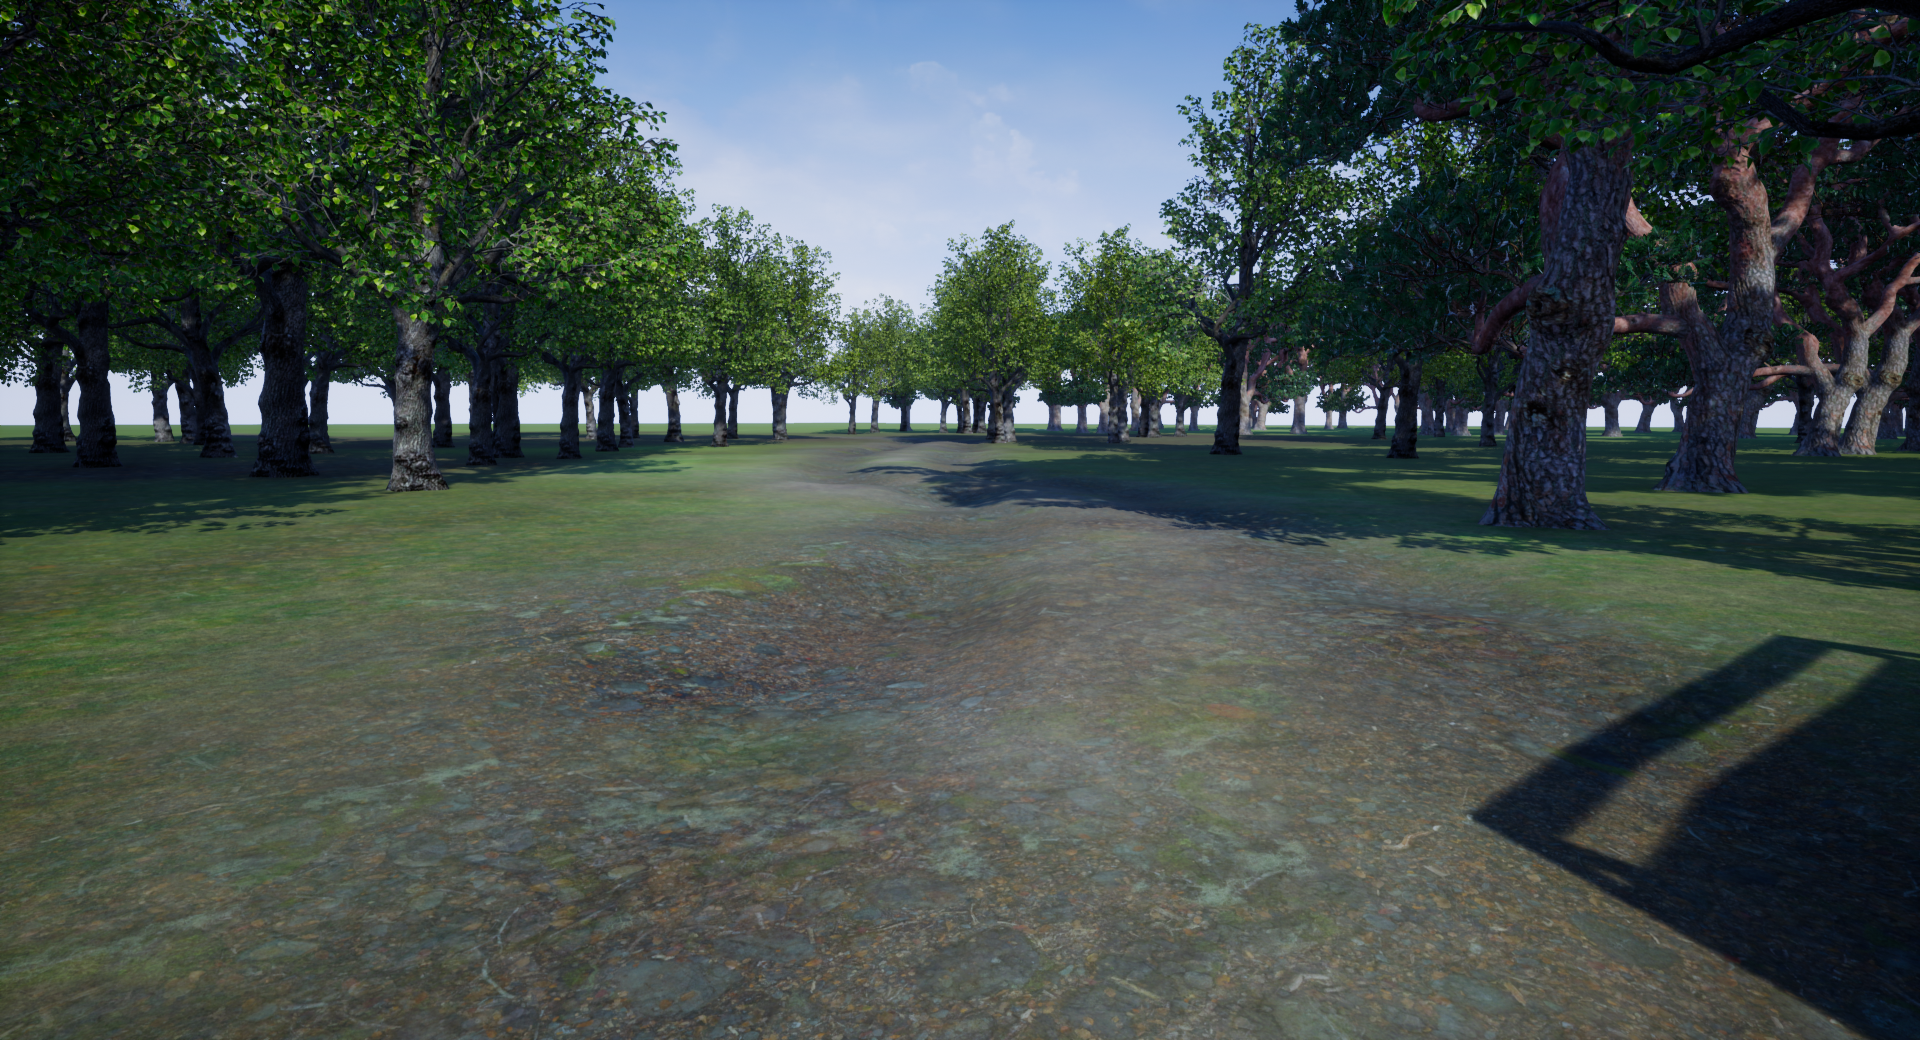
\includegraphics[width=4.5cm]{Chapters/SimulationEnv/Figs/LandscapedVSNotLandscaped/RuttedTrack.png}}\label{fig:RuttedTrack} &


\subfloat[Rail embankment]{\includegraphics[width=4.5cm]{Chapters/SimulationEnv/Figs/LandscapedVSNotLandscaped/RailwayEmbankment.png}}\label{fig:LandscapeMaterialBlueprint} &

\subfloat[Riverbank]{\includegraphics[width=4.5cm]{Chapters/SimulationEnv/Figs/LandscapedVSNotLandscaped/Bridge.png}}\label{fig:LandscapeMaterialBlueprint}

\end{tabular}
\caption{test}
\end{figure}

\subsubsection{Asset Sourcing}
An asset can be described as a piece of content for an Unreal Engine project, which has been serialized to a file. Assets can be re-used and modified in the UE4 editor, but are usually created using external software. UE4 uses assets that come in the Filmbox (.fbx) format, which is a proprietary file format owned by Autodesk\note{Do I need to reference this?}. Conversion tools do exist from other common asset file formats to fbx, but results can vary. Due to limited funding, time and experience, we decided to avoid creating assets from scratch but rather used assets that were free to use. Searching for free assets is a labor-intensive process, as it consisted of a number of steps:
\begin{enumerate}
    \item First, identify possible candidates for a particular type of asset (e.g. a train) based on a search of asset stores that offer free assets. We mainly used \href{https://www.cgtrader.com/}{CGTrader}\footnote{\href {https://www.cgtrader.com/}{https://www.cgtrader.com/}} ,
    
    \href{https://www.turbosquid.com/}{TurboSquid}\footnote{\href {https://www.turbosquid.com/}{https://www.turbosquid.com/}}
    , 
    \href{https://3dwarehouse.sketchup.com/?hl=en}{3D Warehouse}\footnote{\href {https://3dwarehouse.sketchup.com/?hl=en}{https://3dwarehouse.sketchup.com/?hl=en}} 
    and
    \href{https://www.shapenet.org/}{ShapeNet}\footnote{\href {https://www.shapenet.org/}{https://www.shapenet.org/}}.
    
    \item Once a potentially suitable asset had been identified based on it's description and preview, it was downloaded in the Filmbox (fbx) format if possible. Otherwise, it was downloaded in whatever format was available. 
    \item The asset was opened in Autodesk \note{add reference} and visually inspected for suitability. If the textures and geometry were not of a sufficient standard the processes was restarted.
    \item If the asset was deemed suitable from the inspection in Autodesk, then it was exported in Filmbox format.
    \item The asset was then imported into the UE4 editor. Problems often arose in scaling, incorrect texture mapping and one-sided materials applied to the wrong side of assets. These problems could sometimes be addressed; if not we had to restart the process.
\end{enumerate}

\subsubsection{Shadows}
\note{This might not be worth talking about. almost Everything is provided by default}


%Talk about how well static world matches specification, how well rendered images perform for training some object detection etc.
%Also talk about how the environment was packaged and open-sourced with permissive licence for general use



% Not sure of exact ordering here
% 1st Iteration J:\Work\David\ROCSAFEMidTermDemo\Code\UnrealEngine\AirSim\Unreal\Environments\Blocks
% 2nd Iteration J:\Work\David\UnrealEngineRocsafe\OS_01RadIntegr
% 3rd Iteration D:\ROCSAFEScenarios\OS01TestTemp
% 4th Iteration D:\ROCSAFEScenarios\OS_01Radiation - D:\ROCSAFEScenarios\OS_01Radiation\Saved\Screenshots\Windows screenshot 11
% 5th \\ROCSAFE2\ROCSAFEGroupShared\ROCSAFEUnrealEngineOperatingScenarios\NotIntegratedAirSim

% V1: Brussels Demo
% V2: Rail with spline, train, digger. No dirt track, no houses, no road, no wall, poor textures, poor foliage
% V3: Add wall, better foliage
% V4:and houses
% V5: Proper foliage (stones) & blended textures
% V6: Final version in shared folder
